%%%%%%%%%%%%%%%%%%%%%%%%%%%%%%%%%%%%%%%%%%%%%%%%%%%%%%%%%%%
% --------------------------------------------------------
% Tau
% LaTeX Template
% Version 2.4.3 (01/09/2024)
%
% Author: 
% Guillermo Jimenez (memo.notess1@gmail.com)
% 
% License:
% Creative Commons CC BY 4.0
% --------------------------------------------------------
%%%%%%%%%%%%%%%%%%%%%%%%%%%%%%%%%%%%%%%%%%%%%%%%%%%%%%%%%%%

\documentclass[9pt,a4paper,twoside]{tau-class/tau}
\usepackage[english]{babel}

%----------------------------------------------------------
% TITLE
%----------------------------------------------------------

\journalname{Aprenentatge Computacional}
%% TODO: Optional, you can set a fancier title if you like
\title{Classificació tiroidisme}

%----------------------------------------------------------
% AUTHORS, AFFILIATIONS AND PROFESSOR
%----------------------------------------------------------

%% TODO: Set your names here
\author[a,1]{Lluís Panal}

%----------------------------------------------------------

\affil[a]{1668072}

%----------------------------------------------------------
% FOOTER INFORMATION
%----------------------------------------------------------

\institution{Universitat Autònoma de Barcelona}
\footinfo{Class Project}
\theday{Decembre 11, 2024}
\course{Aprenentatge Computacional}

%----------------------------------------------------------
% ABSTRACT AND KEYWORDS
%----------------------------------------------------------

\begin{abstract}    
	%% TODO: Change this default abstract into something nice that describes your work.
	%% Keep it below 300 words.
    Aquest treball es centra en el desenvolupament d'un model d'aprenentatge computacional per a la classificació multiclasse de pacients amb trastorns tiroïdals. L'objectiu principal és predir l'estat de salut d'un pacient en tres categories: sa, amb hipotiroidisme o amb hipertiroidisme, a partir de característiques clíniques i analítiques disponibles. S'analitza diferents maneres de tractar la falta de dades en alguns pacients. El model es basa en tècniques d'aprenentatge supervisat, utilitzant un conjunt de dades amb múltiples variables, com resultats de proves hormonals. S'ha aplicat un conjunt de mètodes de classificació, com Decision Trees o Random Forest, avaluant el rendiment mitjançant la mètrica del f1score. Els resultats obtinguts mostren que el model és capaç de distingir de manera efectiva entre les diferents classes, proporcionant una eina útil per al diagnòstic precoç i la monitorització dels trastorns tiroïdals. \end{abstract}

%----------------------------------------------------------

%% TODO: Set appropriate keywords for your report.
\keywords{a, b, c, d}

%----------------------------------------------------------

\begin{document}
	%% Do NOT change any of this. Line numbers should be kept.
    \maketitle 
    \thispagestyle{firststyle} \tauabstract 
    \tableofcontents
    \linenumbers 
    
%----------------------------------------------------------

\section{Introduction}

    \taustart{E}ls trastorns tiroïdals, com l'hipotiroidisme i l'hipertiroidisme, són condicions mèdiques comunes que afecten un gran nombre de persones a tot el món. Aquests trastorns poden tenir un impacte significatiu en la salut general d'una persona, ja que alteren el funcionament de la glàndula tiroïdal, responsable de regular el metabolisme mitjançant les hormones tiroïdals. El diagnòstic precoç d'aquests trastorns és fonamental per a la prevenció de complicacions greus i per a un tractament adequat. No obstant això, la identificació i classificació de pacients amb trastorns tiroïdals encara pot resultar complexa a causa de la variabilitat dels símptomes i la necessitat d'anàlisis laboratorials detallades.

    L'aprenentatge computacional pot ajudar a detectar de manera automàtica la presència d'aquests trastorns. Així doncs, aquest treball explora l'aplicació d'algoritmes d'aprenentatge supervisat per a la classificació multiclasse de pacients, amb l'objectiu de desenvolupar un model capaç de diferenciar entre els pacients sans i els que tenen alguna alteració de la glàndula tiroïdal.

\section{Exploratory data analysis}
    Les dades han sigut obtingudes a través del \href{https://www.kaggle.com/datasets/emmanuelfwerr/thyroid-disease-data/data}{kaggle}. Aquest dataset conté una sèrie de dades clíniques i analítiques així com el diagnòstic obtingut

    El dataset conté 9172 observacions i cadascuna té 31 atributs, dels quals n'hi ha 20 que són booleans, 8 que són numèrics i 3 que són categòriques (una és el sexe, que es pot passar a binària fàcilment). 
    
    La variable target és una de les de tipus string. Pot pendre els diferents valors: 
    '-', 'S', 'F', 'AK', 'R', 'I', 'M', 'N', 'G', 'K', 'A', 'KJ', 'L', 'MK', 'Q', 'J','C|I', 'O', 'LJ', 'H|K', 'D', 'GK', 'MI', 'P', 'FK', 'B', 'GI', 'C', 'GKJ', 'OI', 'D|R', 'E'

    La informació del dataset ens indica que si pren $'A', 'B', 'C', 'D'$ el pacient té hipertiroidisme i si pren $'E', 'F', 'G', 'H'$ té hipotiroidisme. Els altres valors indiquen o bé que està sa o bé té diagnosticat altres coses que no tenen a veure amb el tiroidisme. He assignat un 0 si el pacient té hipotiroidisme, un 1 si està sa i un 2 si té hipertiroidisme. Amb aquests canvis tenim 667 mostres amb target 0, 8264 amb un 1 i 241 amb un 2, és a dir, està molt desbalancejat.
    
    Hi ha una variable que és única per pacient i no aporta informació, pacient\_id, que serà eliminada.

    Les dades contenen NaNs en 7 variables diferents: sex, TSH, T3, TT4, T4U, FTI i TBG. Les 6 últimes de la llista, que indiquen els nivells de diferents hormones, tenen relació amb una altra variable (cadascuna en té una de diferent), que diu si s'ha mesurat o no. Si indica que no s'ha mesurat, la variable que analitzem té un NaN. Més endavant veurem dues maneres de tractar-los.

    La figura \ref{fig:figure1} mostra la correlació entre variables que no són les mesures de les hormones ni la indicació de si s'ha mesurat o no. També s'ha eliminat les files on la variable sexe té un NaN, un 3.3\% de les dades. Es pot apreciar que la variable target no té massa correlació amb la resta de variables, la qual cosa no és massa bo. Veurem si té més correlació amb les variables eliminades per a fer la matriu.

    \begin{figure}[H]
		\centering
		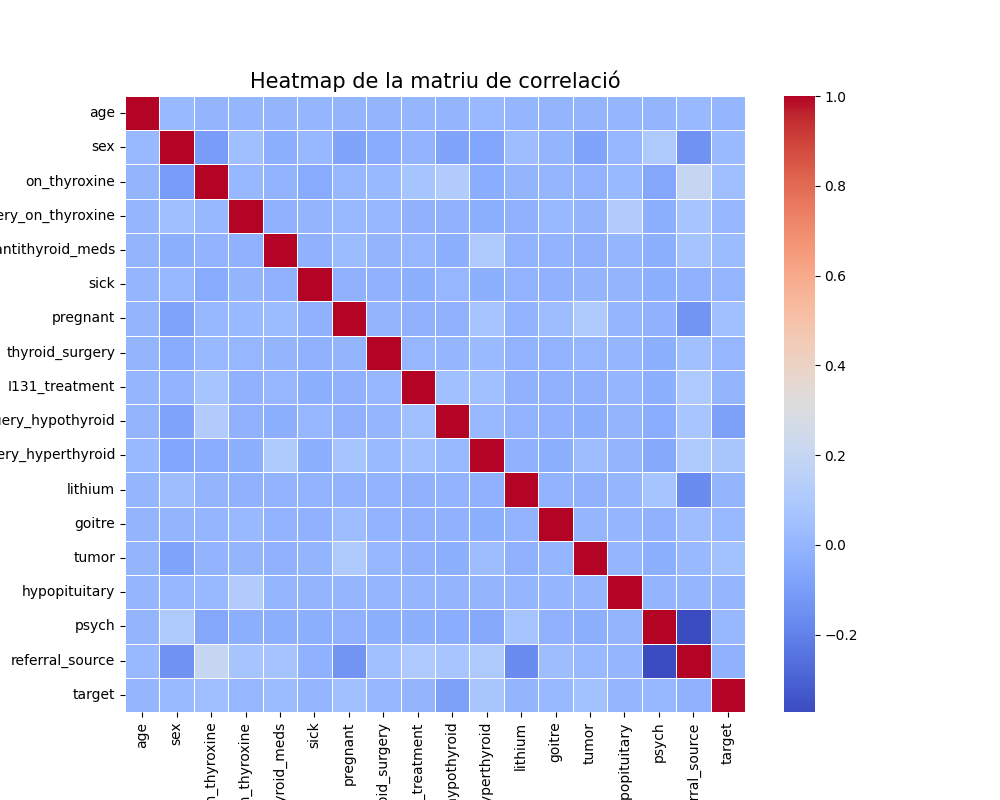
\includegraphics[width=0.75\columnwidth]{correlation_matrix_atributs_no_mesures.png}
		\caption{Matriu de correlació 1.}
		\label{fig:figure1}
	\end{figure}

    La figura \ref{fig:figure2} ens mostra com es distribueix els diagnòstic ens funció de l'edat (amb certes modeificacions que explicaré a l'apartat 3.1) i el sexe. A simple vista no es veu que tingui cap mena de relació.

    \begin{figure}[H]
		\centering
		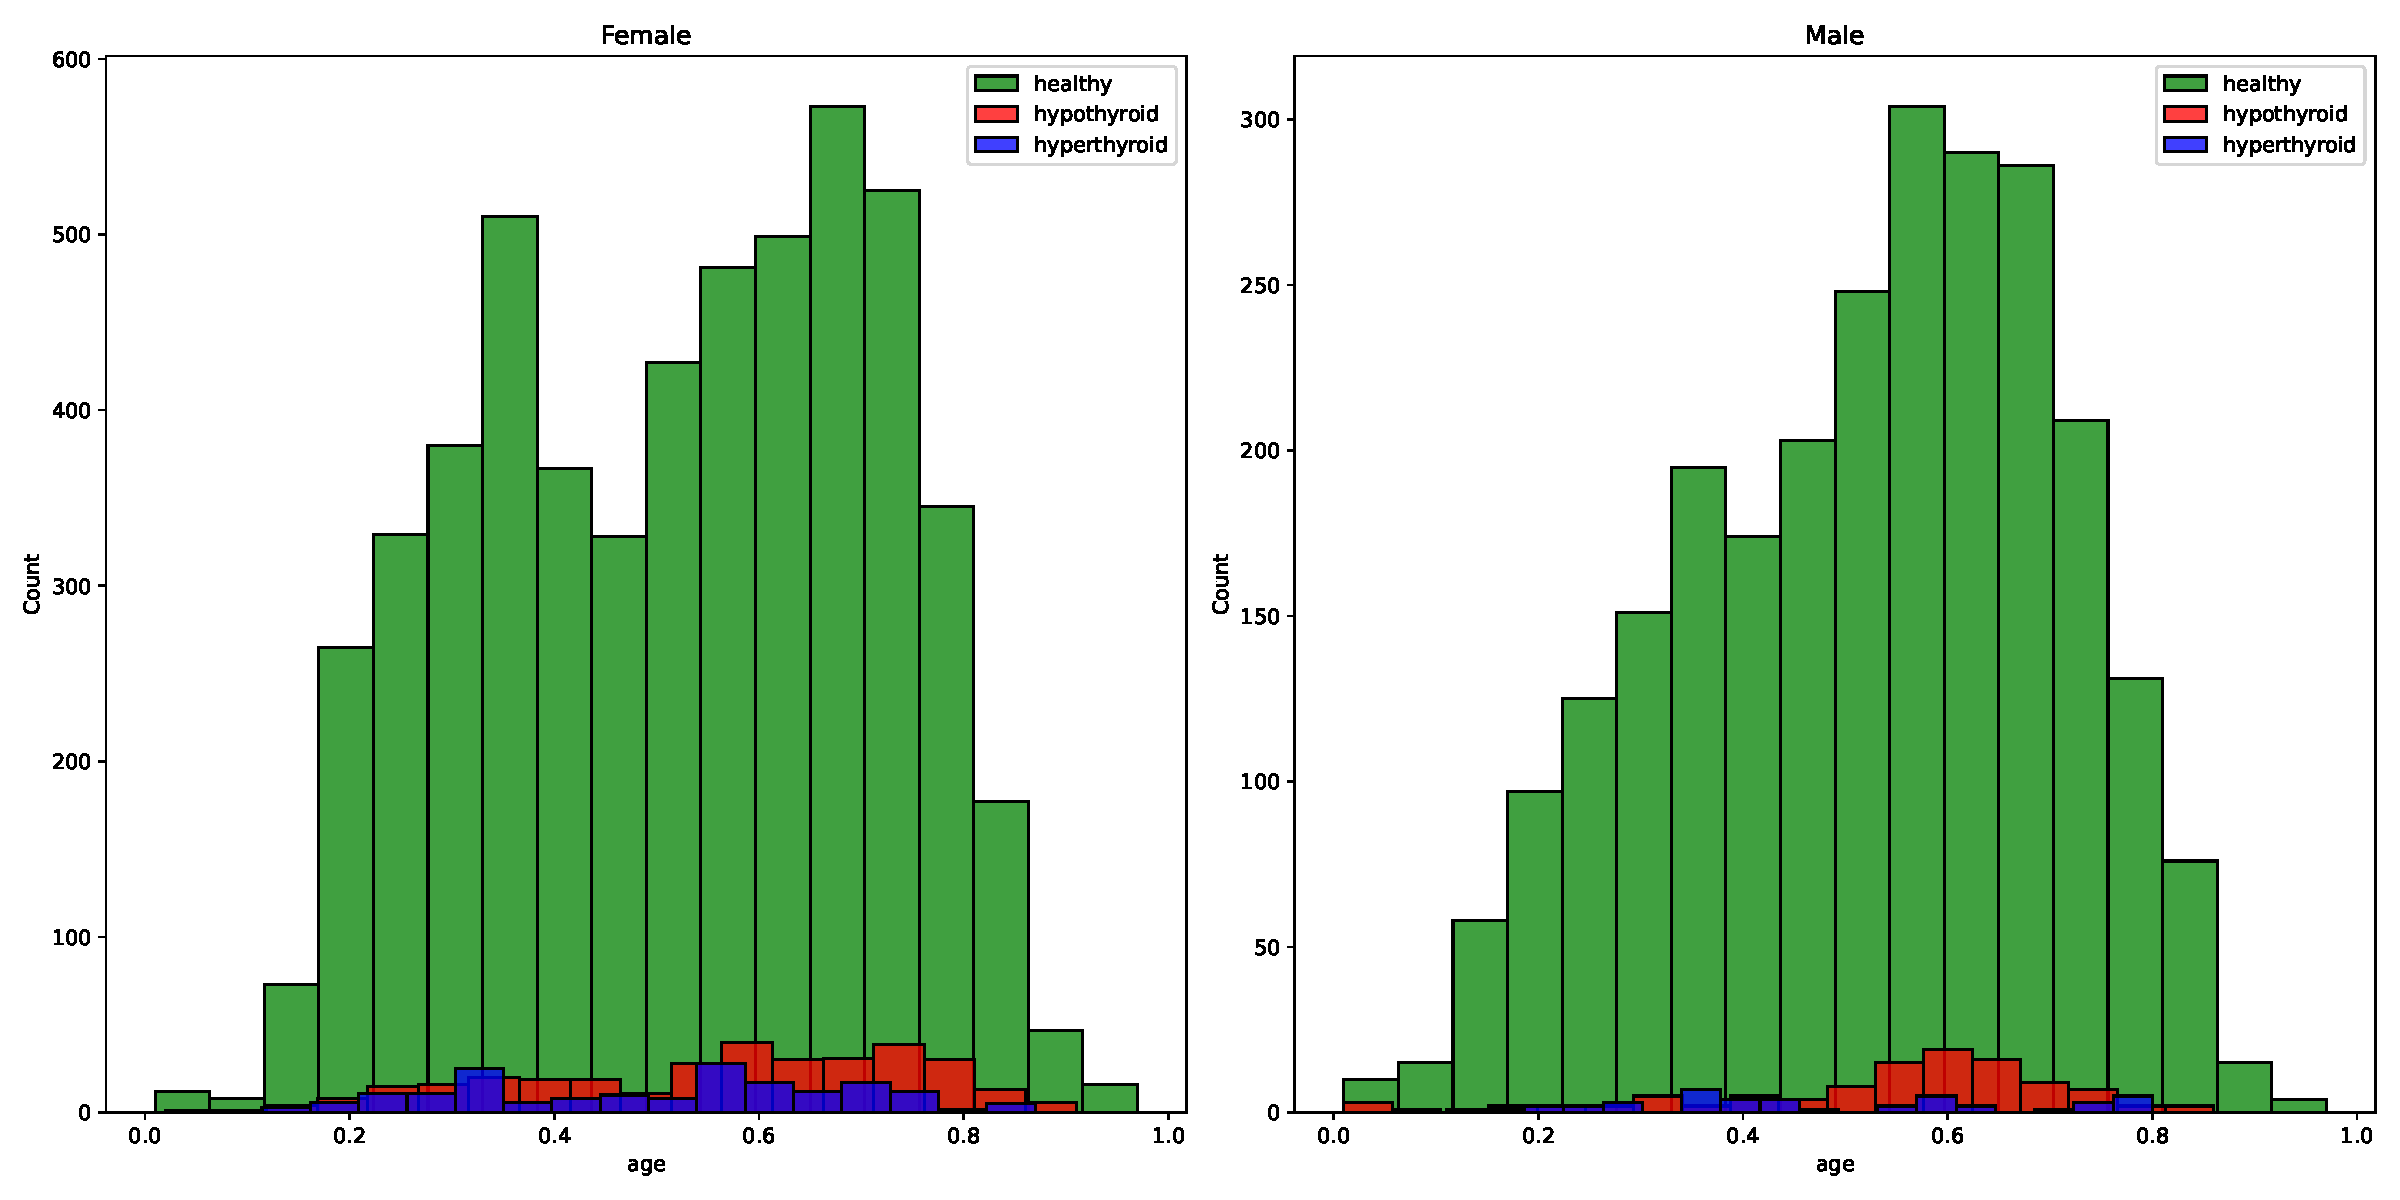
\includegraphics[width=0.75\columnwidth]{relacio_edat_sexe_target.pdf}
		\caption{Relació entre l'edat, el sexe i el target.}
		\label{fig:figure2}
	\end{figure}

    La figura 3 ens mostra les distribucions dels diagnòstics en funció de la font de referència. Aquesta gràfica sí que és més interessant, ja que hi ha dues fonts que mai diagnostiquen com a hipertiroidisme, i una, 'WEST', d'aquestes dues tampoc ho fa amb el hipotiroidisme, és a dir, diu que tothom està sa. Això passa en part perquè només hi ha 3 dades amb aquesta font.
    \begin{figure}[H]
		\centering
		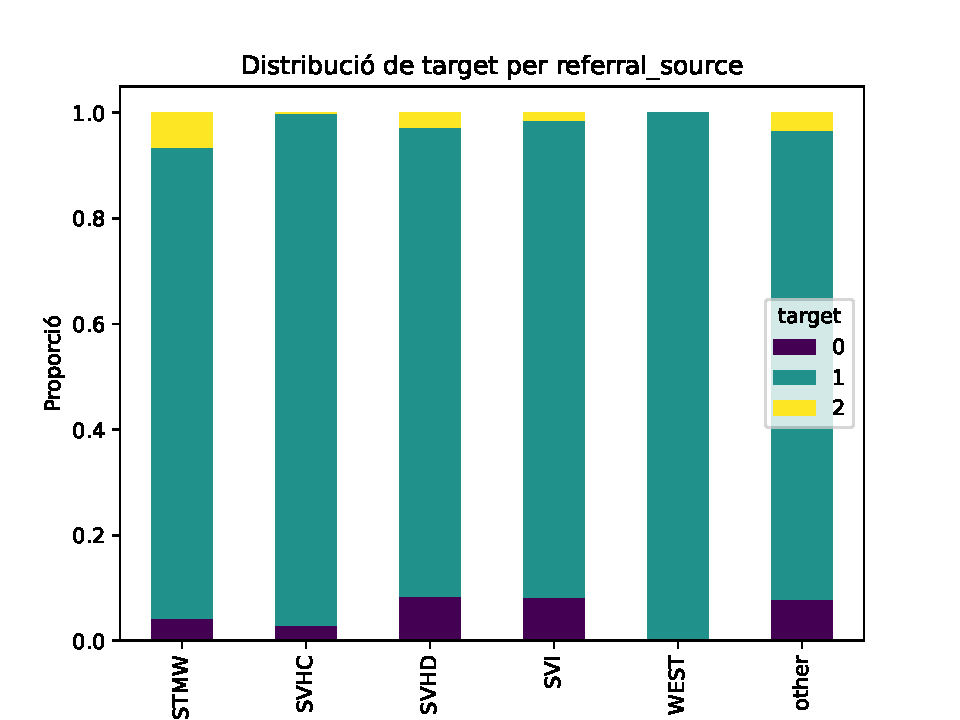
\includegraphics[width=0.75\columnwidth]{proporcio_referral_source_target.pdf}
		\caption{Relació entre referral source i el target.}
		\label{fig:figure3}
	\end{figure}

\section{Preprocessing}

    Abans que res, vull destacar que no normalitzaré perquè al haver-hi dades mèdiques no vull perdre el seu significat.

    A continuació explicaré com he tractat diferents problemes que portaven algunes de les variables.
    \subsection{'age'}
    D'aquesta en principi sembla tot correcte ja que no hi ha NaNs ni valors negatius, però si mirem les dades que prenen el valor màxim veiem que hi ha quatre mostres que tenen molt més de 100 anys. No sé si és que no se sabia l'edat o un error humà al agafar la dada, així que com que només eren 4 mostres les he eliminat. Més endavant li faré algun retoc més.

    \subsection{'referral\_source'}
    Aquí més que un problema és que s'ha hagut de passar de categòrica a numèrica. Per a fer-ho he creat tantes variables binàries com opcions n'hi ha, 5. D'aquestes he eliminat la que menys n'hi ha, 'WEST', ja que la informació es pot obtenir de les altres variables.

    \subsection{'sex'}
    Aquí sí que hi ha un problema: els NaNs. La variable té un 3,3\% de NaNs. Només hi ha una manera que ens permeti omplir algunes files: mirar si el pacient està embarassat. Malauradament això només omple 4 files. Com que és només un 3\% i la distribució no s'altera notablement, he decidit eliminar les files. Ara tenim 7998 amb target 1, 642 amb 0 i 225 amb 2

    \subsection{Nivells hormonals}
    Com he comentat anteriorment, per a cada indicador hi ha dues variables: una que indica si s'ha mesurat o no i l'altres que dona la mesura si l'altre és positiva o té un NaN si l'altre és negativa. No hi ha cap NaN que en files on sí que s'hagi mesurat, per això he eliminat les columnes que indiquen si s'ha mesurat o no. Com que si mirem totes les files que tenen un NaN en alguna de les sis columnes em quedaria sense dades, no les puc eliminar, les he d'omplir. Ho he provat de dues maneres diferents.

    \subsubsection{Canviar els Nans per -1}
    Aquesta estratègia pot arribar a ser útil en models no massa simples, no pot funcionar amb una regressió logística, per exemple, ja que intentaria predir amb aquest valor de la mateixa manera que amb qualsevol altre. Un altre problema que pot portar és que no tots els indicadors tenen la mateixa escala, és a dir, no és el mateix per un indicador que pot pendre valors entre 0 i 10 que per una altra que pot prendre valors entre 0 i 1000. L'escala de les dades també pot ser un problema per un altre motiu: al tenir escales diferents per a les variables, pot ser que afecti als paràmetres de manera que no només tinguin en compte la importància. Per això el que vaig fer va ser dividir cada indicador per el valor màxim que està considerat com a sa, d'aquesta manera tot quedava a escales similars. A més a més, el -1 ara és prou petit (gran negativament) com per a separar-se de les mostres. La figura \ref{fig:figure4} mostra la matriu de correlació entre aquestes variables i el target
    \begin{figure}[H]
		\centering
		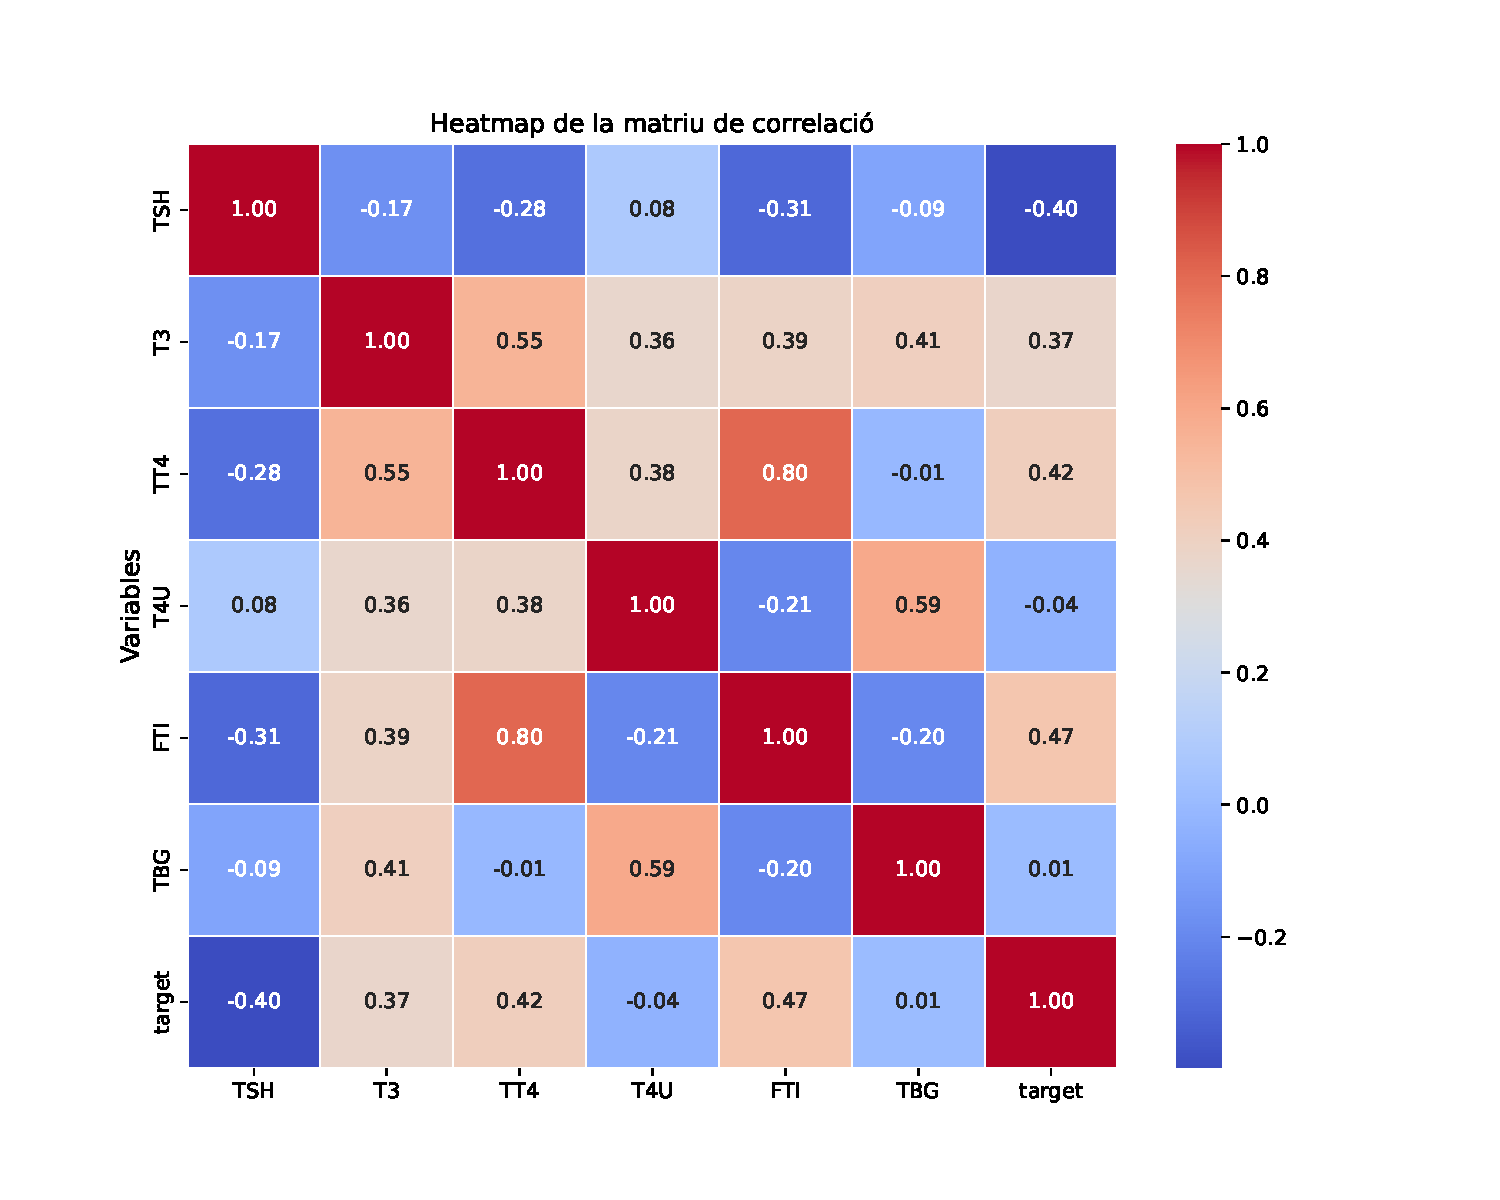
\includegraphics[width=0.75\columnwidth]{correlation_matrix_atributs_df_fillna.pdf}
		\caption{Matriu de correlació entre les mesures d'indicadors.}
		\label{fig:figure4}
	\end{figure}

    Aquí sí que hi ha variables que tenen correlació amb el target, com el TSH, que pot ser útil.

    Ara només l'edat pren nombres molt grans en comparació a la resta. Com que només hi ha edats entre 1 i 100 anys, la vaig dividir entre 100 per a tenir-les amb un rang entre 0 i 1 a una escala similar a les altres variables.

    \subsubsection{Discretitzar els indicadors}
    La segona opció va ser separar els valors en intervals, de manera que si hi havia una mesura feta la fila tindria un 1 en un dels intervals i un 0 en els altres, i si, en canvi, hi hagués un NaN, tots els intervals tindrien un 0. La opció final que he triat ha sigut fer 3 intervals, un pels que tenen un valor baix, un pels que tenen un valor normal i un últim pels que tenen un valor alt. Els llindars per a determinar a cada interval pertany cada pacient els he buscat. He trobat els següents:
    \begin{itemize}
        \item TSH: 0.26, 5.6
        \item T3: 1.8, 4.6
        \item TT4: 60, 150
        \item T4U: 0.7, 1.3
        \item FTI: 60, 150
        \item TBG: 13, 39
    \end{itemize}

    Vull destacar que també vaig provar de separar-ho en 6 intervals, separar cadascun dels 3 anteriors en dos. Els resultats obtinguts eren lleugerament inferiors, així que ho vaig descartar. Una de les causes podria ser que aquests nous llindars els vaig posar de manera arbitrària, ja que no hi havia cap criteri oficial.

    Amb aquesta manera de tenir en compte els NaNs, l'única variable que ara no és binària és l'edat. Així doncs, també la vaig discretitzar en 6 intervals. Ara doncs, totes les variables són binàries.

    La figura \ref{fig:figure5} mostra la correlació entre les noves variables i el target
    \begin{figure}[H]
		\centering
		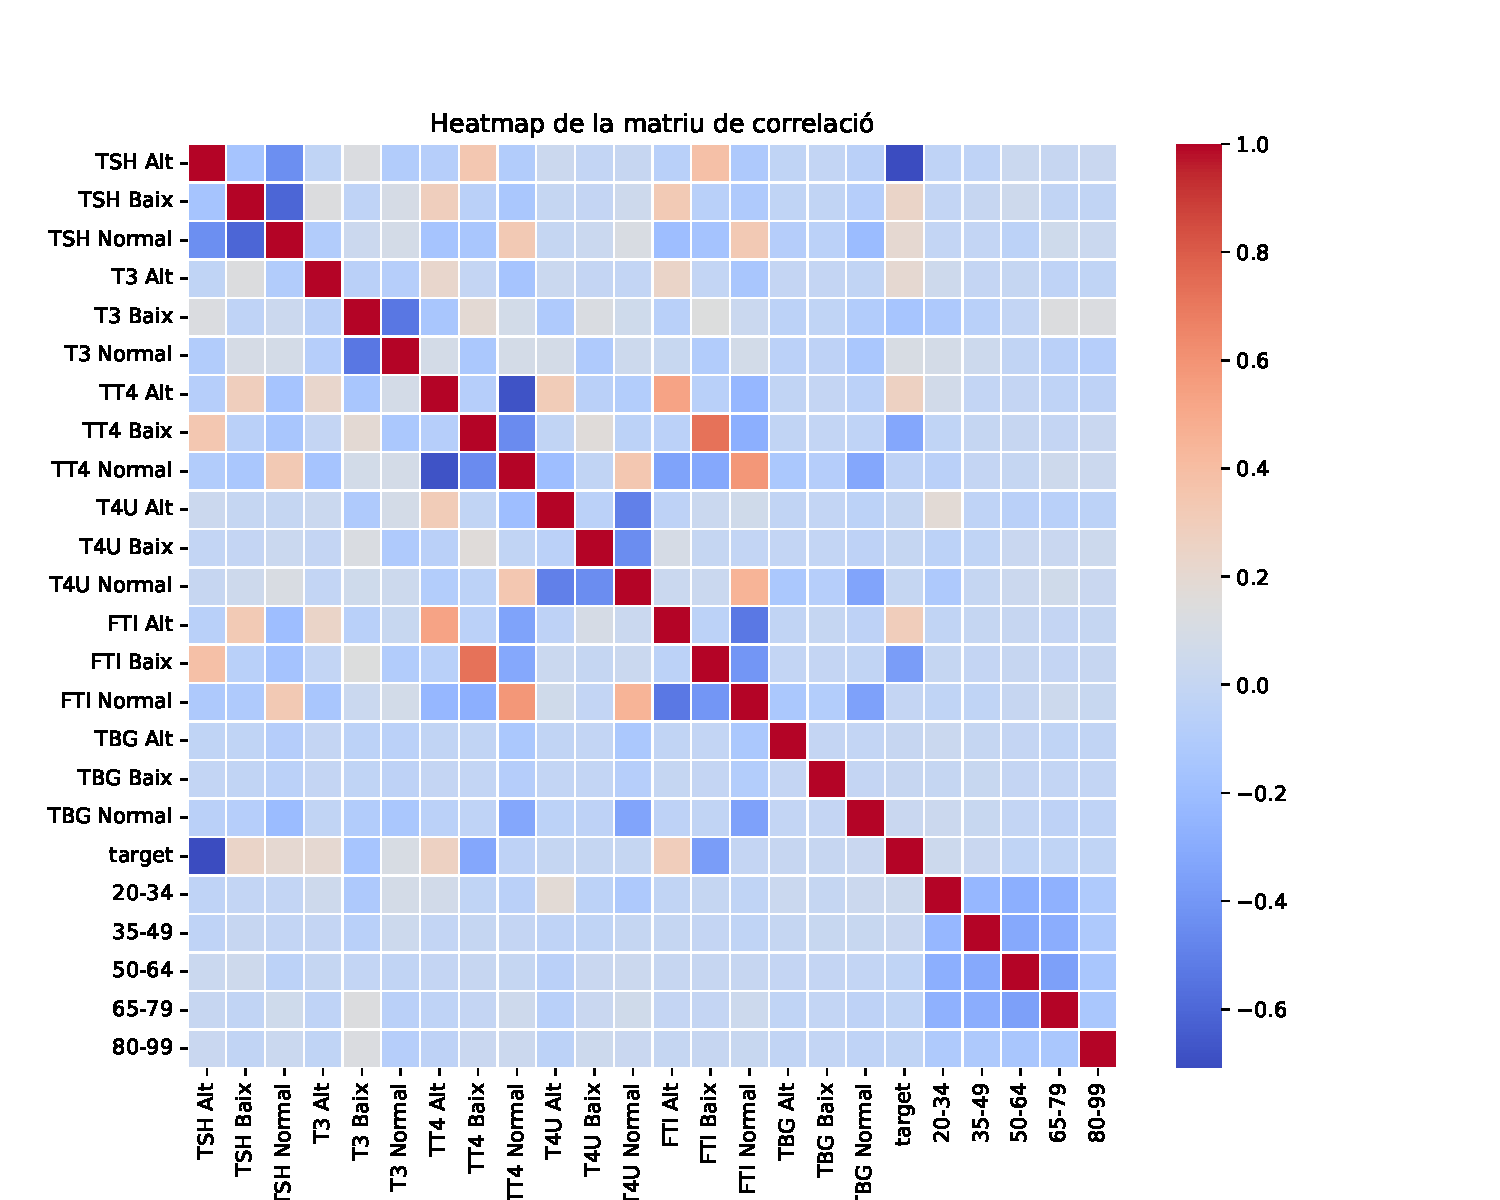
\includegraphics[width=0.75\columnwidth]{correlation_matrix_atributs_df_intervals.pdf}
		\caption{Matriu de correlació entre les variables d'intervals.}
		\label{fig:figure5}
	\end{figure}

    Aquí també hi ha algunes variables que tenen una forta correlació amb el target.

    A partir d'aquí aniré distingint entre les dues opcions d'omplir els NaNs (en la notebook primer es fa l'estudi de les dades omplint NaNs i després l'estudi de la versió d'intervals).

    Com que ja he acabat amb el tractament de les variables, a partir d'ara separaré un 10\% de les dades per a fer el test final. L'altre 90\% em servirà per a fer els entrenaments i les cerques d'hiperparàmetres.

    \subsection{PCA}
    En aquest punt em va sorgir el dubte de si tenia moltes variables, i si això em podria causar overfitting. Per això vaig provar de fer una primera validació creuada i vaig fer un entrenament amb un gradient boosting amb els paràmetres per defecte. Els resultats donen una aproximació del resultat real, és a dir, pot ser que aquest split sigui molt bo i els resultats siguin una mica superiors, però també pot ser dolent i donar ser una mica inferior.
    La metrica està explicada més endavant. Vaig obtenir el següent:
    \begin{itemize}
        \item Omplir amb -1
        \item \begin{itemize}
            \item Train: 0.97
            \item Validació: 0.90
        \end{itemize}
        \item Intervals
        \item \begin{itemize}
            \item Train: 0.91
            \item Validació: 0.87
        \end{itemize}
    \end{itemize}
    Com que els resultats de la validació no són molt inferiors al dels train no considero que hi hagi overfitting. Tot i això vaig voler provar de fer un PCA, per veure si amb una dimensionalitat molt més baixa es també es podria fer i l'entrenament seria menys costós.

    En fer les representacions no es semblan gaire separables i si fem un entrenament, el rendiment és inferior a 0.7 per les dues opcions.
    Les figures \ref{fig:figure6} i \ref{fig:figure7} mostren els dos PCA.
    \begin{figure}[H]
		\centering
		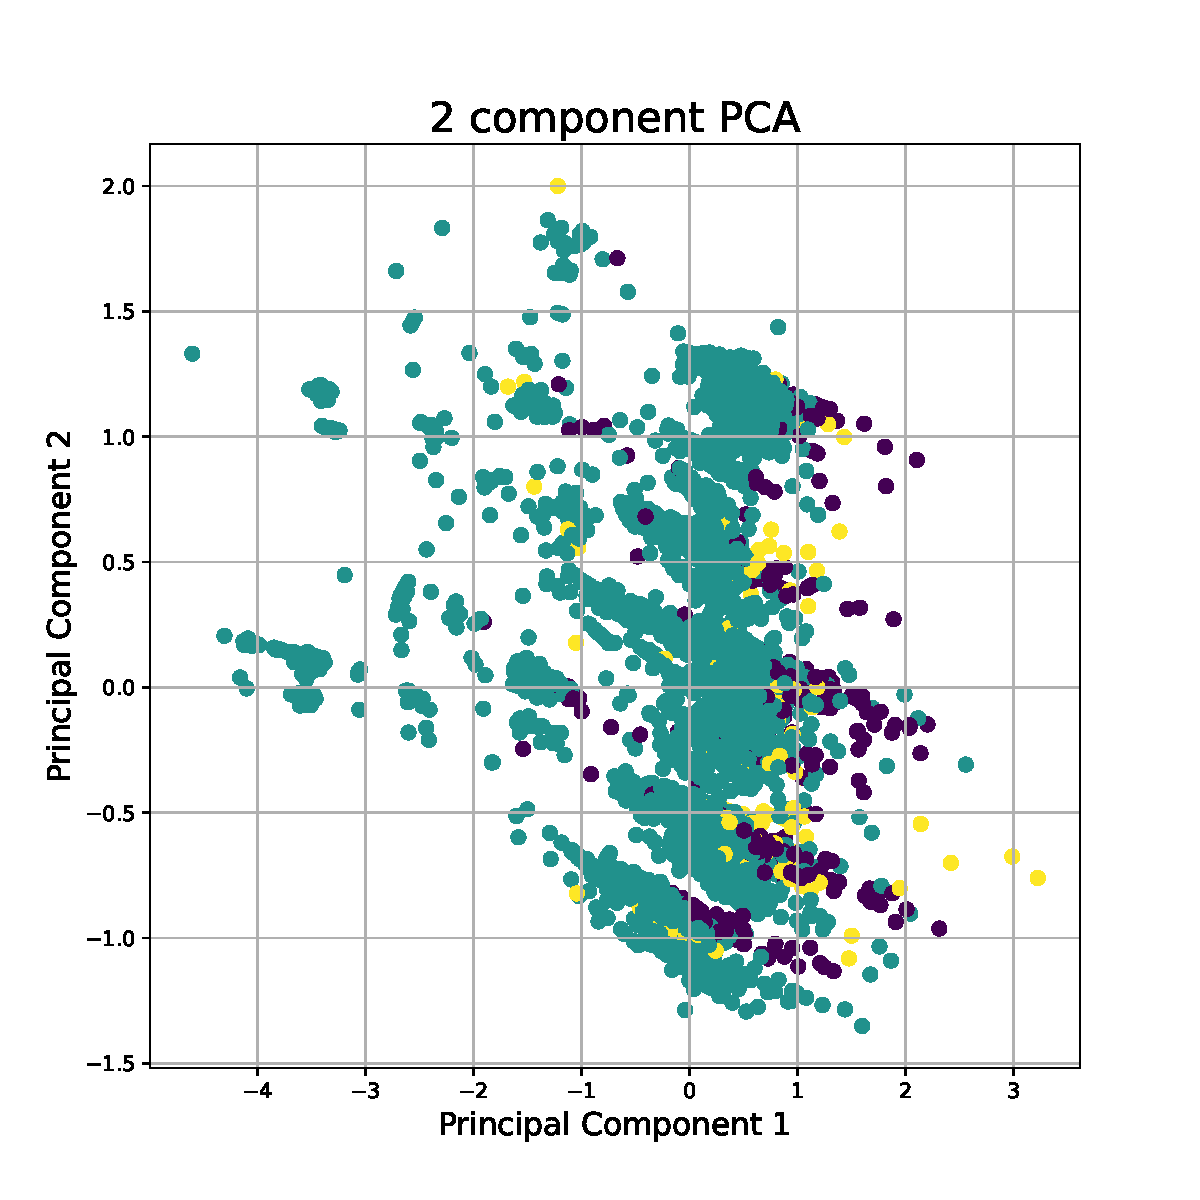
\includegraphics[width=0.75\columnwidth]{PCA_df_fillna.pdf}
		\caption{PCA omplint amb -1.}
		\label{fig:figure6}
	\end{figure}\begin{figure}[H]
		\centering
		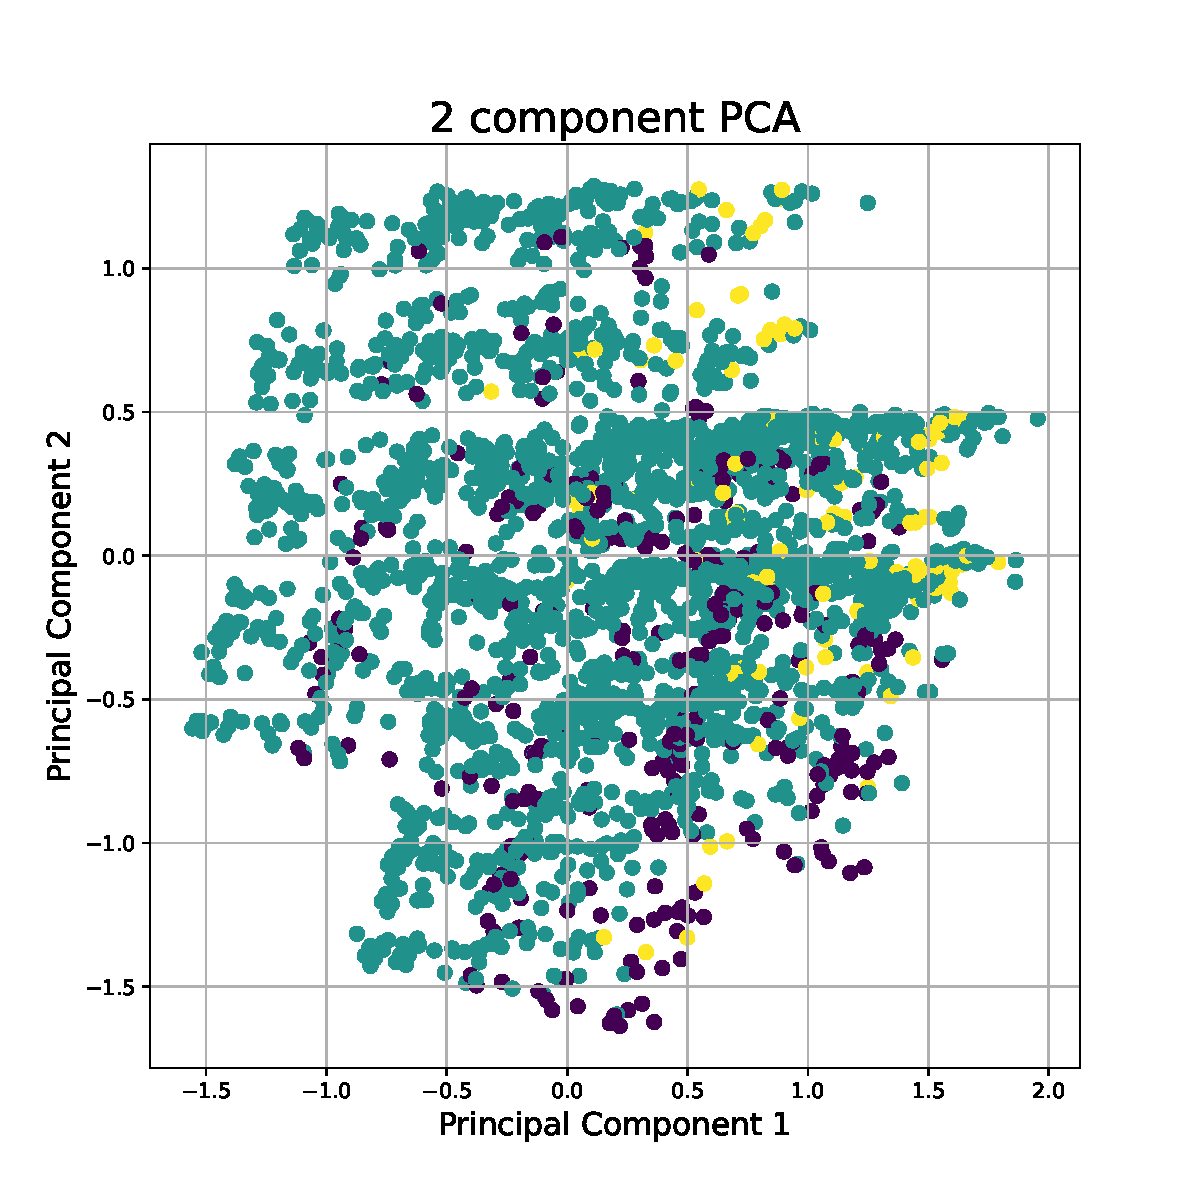
\includegraphics[width=0.75\columnwidth]{PCA_df_intervals.pdf}
		\caption{PCA passant a intervals.}
		\label{fig:figure7}
	\end{figure}

    Més endavant també provaré d'agafar les features que tenen més importància dins de cada model.

    \section{Mètrica}
    Com que el meu dataset és molt desbalancejat, hi ha 8264 pacients sans, 667 pacients amb hipotiroidisme i 241 pacients amb hipertiroidisme, la mètrica que utilitzaré serà el f1 score. A més a més, l'average utilitzat és 'macro', d'aquesta manera, totes les classe tenen el mateix pes independenment de la quantitat de mostres que hi hagi de la classe.
    En alguns llocs, com en el resultat final, també mostraré l'accuracy, tot i que no el tindré tant en compte.


    \section{Selecció de model}
    Models utilitzats:
    \begin{itemize}
        \item Logistic regression: Un dels models més senzills, intuïtius i ràpids per a la classificació binària, que es basa en una funció logística per predir la probabilitat d'una classe.
        \item SVC (Support Vector Classifier): Extremadament efectiu en espais de gran dimensió o quan les classes no són linealment separables, ja que busca el millor marge per separar les classes.
        \item KNN (K-nearest neighbors): Un mètode senzill que no requereix entrenament previ, i classifica les dades basant-se en la classe dels veïns més propers a un punt donat.
        \item Decision tree: Un model senzill que divideix iterativament l'espai de característiques en subgrups, sent fàcil d'interpretar i visualitzar.
        \item Random forest: Un conjunt de decision trees que ajuda a reduir l'overfitting mitjançant la creació de múltiples arbres i la mitjana dels seus resultats, millorant així la robustesa del model.
        \item Gradient Boosting: Una tècnica d'ensemble que combina diversos models febles per crear un model fort, optimitzant l'error de forma iterativa mitjançant un algorisme de reforç de gradients per millorar les prediccions.
        \item XGBoost: Una implementació eficient i altament optimitzada del gradient boosting, que inclou tècniques de regularització i altres millores per prevenir l'overfitting i augmentar la precisió del model.
    \end{itemize}
    He de destacar que tant la regressió logística com el SVC no són capaços de realitzar una classificació multiclasse de manera directa, ja que estan dissenyats per a problemes de classificació binària. És per això que per aquests dos models dues estratègies: One-vs-One (OVO) i el One-vs-Rest (OVR). L'OVO consisteix a crear un classificadors per a cada parell de classes possibles, de manera que, en el cas de 3 classes, es creen 3 classificadors. En canvi, l'OVR crea un classificador per a cada classe, intentant distingir una classe contra totes les altres, el que també genera 3 classificadors. La resta de models poden gestionar la classificació multiclasse directament sense necessitat d'estratègies addicionals.

    Primer he fet un avaluació dels models amb els paràmetres per defecte, utilitzant 10 splits independents. Les figures \ref{fig:figure8} i \ref{fig:figure9} mostra els resultats:
    \begin{figure}[H]
        \centering
        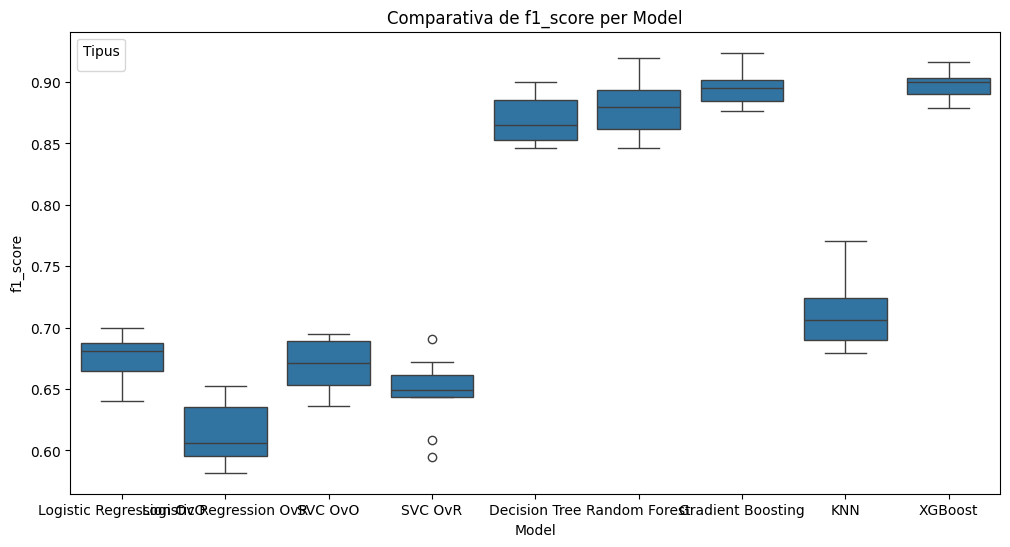
\includegraphics[width=0.75\columnwidth]{parametres_per_defecte_df_fillna.png}
        \caption{Resultats dels models inicialitzats per defecte amb el dataset d'omplir amb -1.}
        \label{fig:figure8}
    \end{figure}
    Com era previsible, tant la regressió com el SVC no han obtingut un resultat massa bo. El SVC el descartaré per la cerca d'hiperparàmetres, ja que és força costós i no ha obtingut un resultat gaire bo. La regressió sí que la deixaré perquè és força simple i no gasta gaire temps.

    \begin{figure}[H]
        \centering
        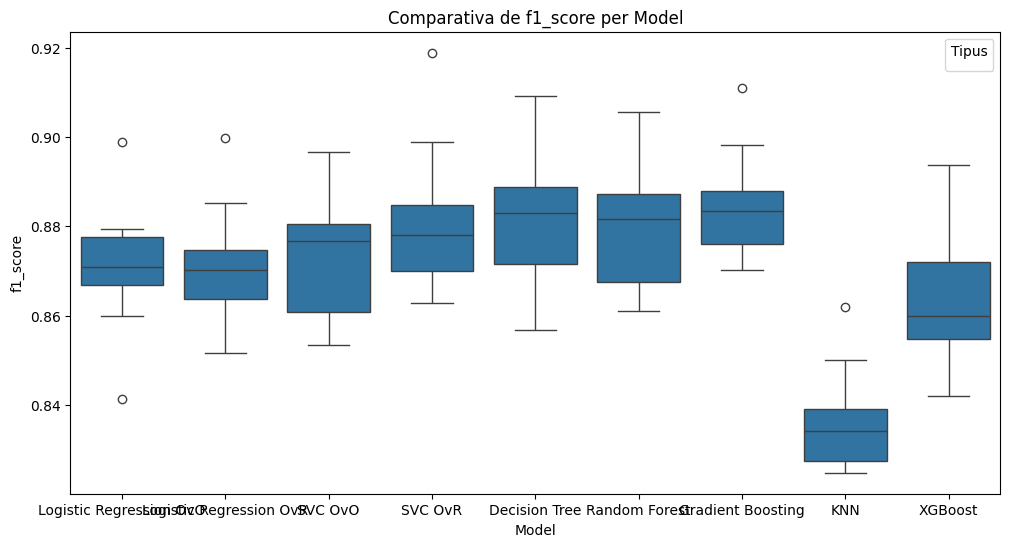
\includegraphics[width=0.75\columnwidth]{parametres_per_defecte_df_intervals.png}
        \caption{Resultats dels models inicialitzats per defecte amb el dataset d'intervals.}
        \label{fig:figure9}
    \end{figure}
    Tot i que aquí el decision tree és el que ha tret millors resultats en mitjana, els altres models no s'han quedat gaire lluny. Els resultats d'aquest dataset són una mica inferiors als millors models de l'altre, així que seguiré provant de les dues maneres.

    Com he dit abans tinc moltes variables en el model. Una altra manera de reduir aquest nombre és seleccionar només les més importants. En fer-ho m'ha seleccionat les següents features:
    \begin{figure}[H]
        \centering
        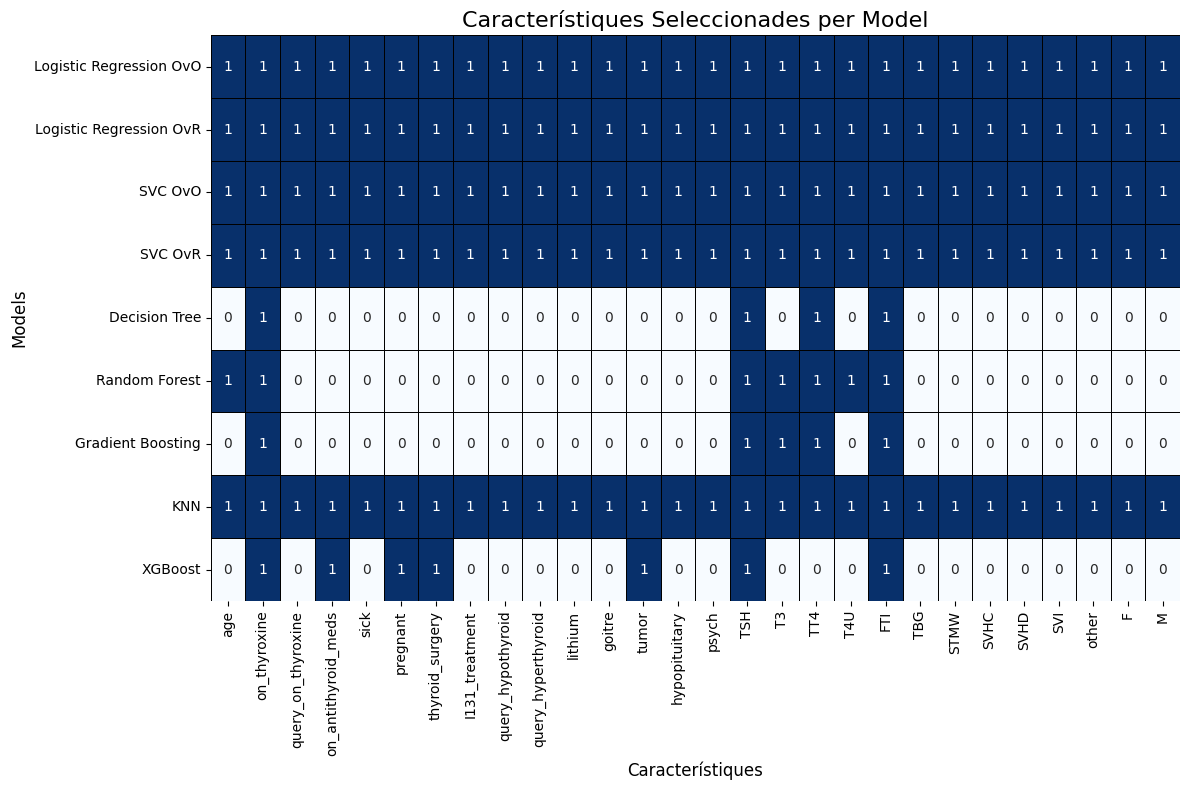
\includegraphics[width=0.75\columnwidth]{selected_features_df_fillna.png}
        \caption{Variables seleccionades del dataset omplint amb -1.}
        \label{fig:figure10}
    \end{figure}
    \begin{figure}[H]
        \centering
        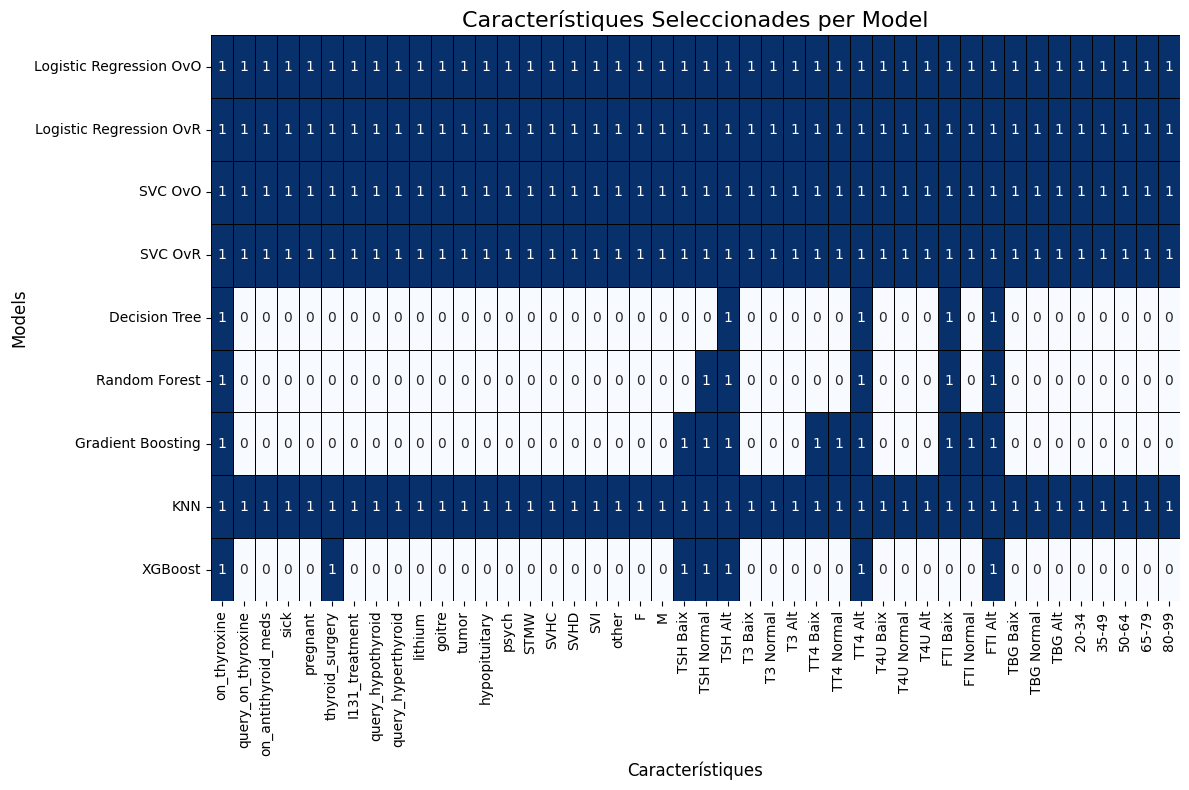
\includegraphics[width=0.75\columnwidth]{selected_features_df_intervals.png}
        \caption{Variables seleccionades del dataset d'intervals.}
        \label{fig:figure11}
    \end{figure}

    Malauradament tant el knn com el OneVsOne i el OneVsRest no tenen la opció de seleccionar features.

    Amb aquests models i les variables que han seleccionat cadascun obtenim un resultat lleugerament inferior a fer-ho amb totes. Tot i així faré també la cerca d'hyperparametres.

    A continuació vaig realitzar la cerca d'hiperparàmetres. Per a fer-ho he utilitzat 10 K-folds i la funció GridSearch. La figura \ref{fig:figure12} mostra les mitjanes dels f1 scores que ha obtingut el model amb els millors hyperparàmetres.


    \begin{figure}[H]
        \centering
        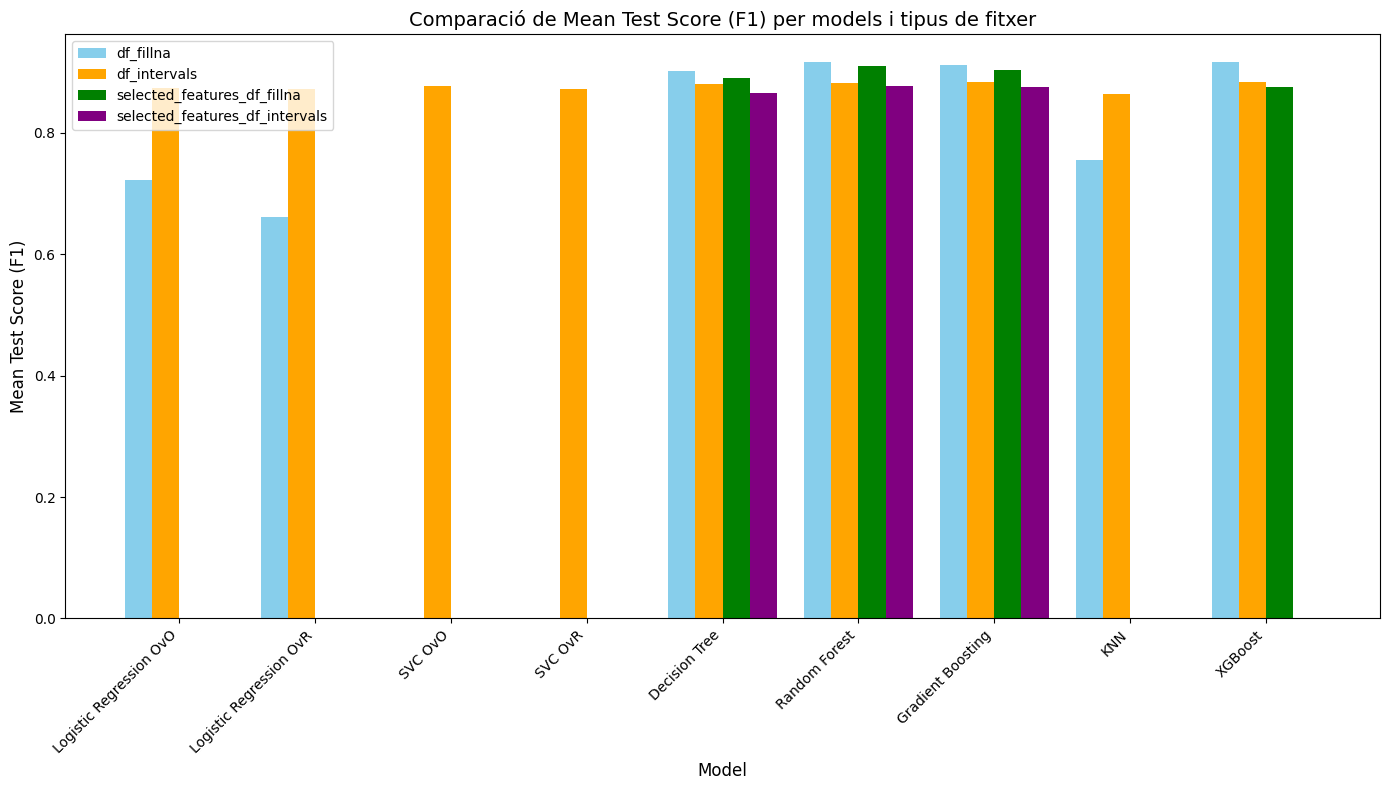
\includegraphics[width=0.75\columnwidth]{millors_hyperparametres.png}
        \caption{F1 scores dels models amb els millors hyperparàmetres.}
        \label{fig:figure12}
    \end{figure}
    
    \section{Resultats}

    El millor model ha sigut aquest: $RandomForestClassifier(criterion='entropy', max_features=None,
    min_samples_leaf=2, min_samples_split=10,
    random_state=20)$, omplint els NaNs amb un -1.

    Ara el podem entrenar amb totes les dades d'entrenament i validació i comprovar la seva eficàcia amb les dades reservades. Resultats:
    \begin{itemize}
        \item F1 score: 0.949
        \item Accuracy: 0.988
    \end{itemize}
    I obtenim la matriu de confusió segünet:
    \begin{figure}[H]
        \centering
        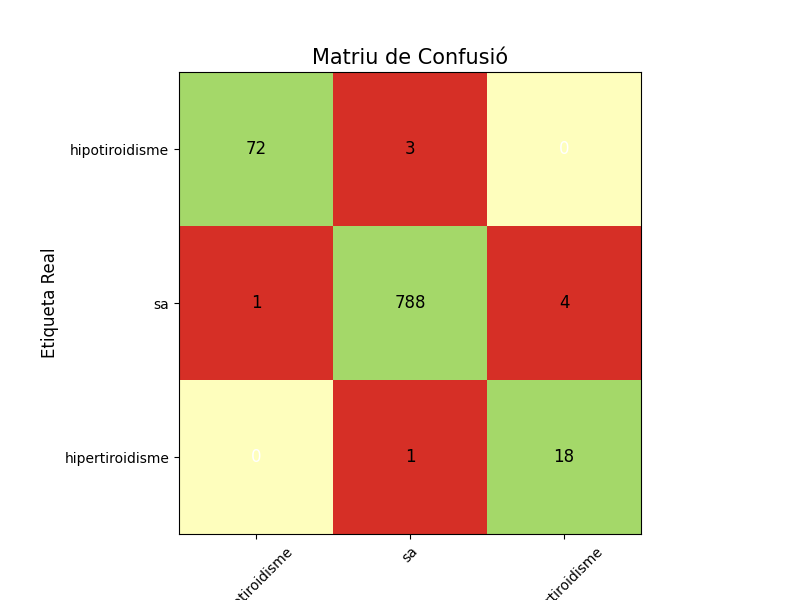
\includegraphics[width=0.6\columnwidth]{confusion_matrix_best_model.png}
        \caption{Matriu de confusió del millor model.}
        \label{fig:figure13}
    \end{figure}
    Per la matriu podem veure que el model prediu força bé i per això ha obtingut un f1 score tant alt. Vull destacar dues coses: la primera és que el model no s'equivoca entre hipertiroidisme i hipotiroidisme, i la segona és que prediu millor l'hipotiroidisme que l'hipertiroidisme, probablement perquè la segona és minoritària.
    Si mirem el classification report ens indica el següent:
    \begin{table}[h]
        \centering
        \begin{tabular}{lcccc}
        \toprule
         \textbf{Classe} & \textbf{Precision} & \textbf{Recall} & \textbf{F1-Score} & \textbf{Support} \\
        \midrule
        \textbf{Hipotiroidisme} & 0.99 & 0.96 & 0.97 & 75 \\
        \textbf{Sa} & 0.99 & 0.99 & 0.99 & 793 \\
        \textbf{Hipertiroidisme} & 0.82 & 0.95 & 0.88 & 19 \\
        \bottomrule
        \end{tabular}
        \caption{classification report.}
        \label{tab:classification_results}
    \end{table}
        


    \section{Conclusions}
    A partir de l'anàlisi i el desenvolupament del model per a la classificació de pacients amb trastorns tiroïdals, es poden extreure les següents conclusions:
    \begin{itemize}
        \item Preprocessament de Dades: El tractament de dades mancants va ser crucial per a la creació del model. Les dues tècniques provades per omplir els valors faltants (omplir amb -1 o discretitzar els valors en intervals) van mostrar resultats molt bons. To t i que a mi personalment em semblaria millor la versió dels intervals, ha sigut l'altre la millor.
        \item Els models més complexos són els que han obtingut millors resultats. Els més simples, la regressió i el SVC, ha tingut problemes, sobretot amb l'estratègia d'omplir amb -1, degut a la seva naturalesa.
        \item Tot i haver provat diferents estratègies per a reduir el nombre de variables, amb un PCA o triant les més importants, el millor ha sigut treballar amb totes elles.
    \end{itemize}

    Per aconseguir millora encara una mica més es poden provar diferents coses:
    \begin{itemize}
        \item Per a la versió d'omplir els NaNs amb -1 es pot provar d'omplir després d'escalar amb un valor molt gran, com per exemple 100, així el NaN tindria un efecte diferent.
        \item Per a la versió d'intervals es pot provar de fer-ho amb 6 intervals com he comentat, però els threshold han de tenir una justificació mèdica.
        \item També es podria establir uns llindars en funció de l'edat
        \item Provar algun hyperparametre més, sobretot en el random forest i el gradient boosting, que han tret les majors puntuacions.
    \end{itemize}

    \begin{thebibliography}{9}

        \bibitem{vaswani_attention_2017}
        Emmanuel Fwerr,
        \textit{Thyroid Disease Data},
        Kaggle, 2017.
        Disponible a: \url{https://www.kaggle.com/datasets/emmanuelfwerr/thyroid-disease-data}
        
        \bibitem{PFGPlots}
        Cigna Health,
        \textit{Pruebas de hormona tiroidea},
        Cigna Knowledge Center, 2024.
        Disponible a: \url{https://www.cigna.com/es-us/knowledge-center/hw/pruebas-mdicas/pruebas-de-hormona-tiroidea-hw27377}

        \bibitem{cun_tiroidea_es}
        Clínica Universidad de Navarra,
        \textit{Pruebas de función tiroidea},
        Disponible a: \url{https://www.cun.es/enfermedades-tratamientos/pruebas-diagnosticas/funcion-tiroidea}

        \bibitem{cun_tiroidea_en}
        Clínica Universidad de Navarra,
        \textit{Thyroid Function Tests},
        Disponible a: \url{https://www.cun.es/en/diseases-treatments/diagnosis-procedures/function-thyroid}

        \bibitem{medlineplus}
        MedlinePlus,
        \textit{Thyroid Function Tests},
        Disponible a: \url{https://medlineplus.gov/ency/article/003374.htm}

    \end{thebibliography}



\end{document}